\chapter{Related Work}
\label{cha:related-work}
\epigraph{We should think of the compiler as being our lab assistant.}{Edwin Brady}

\noindent
Following Edwin Brady's philosophy of compilers being our lab assistants, this section will provide an overview of existing solutions targeting the problem of rotting todo comments as well as existing implementations of hole-driven development.
After presenting these existing implementations, we will highlight established, novel, and creative workarounds and alternatives for simulating holes in broadly used languages.
This chapter will conclude with a list of properties intrinsic to managing todo-comments as well as working with holes while developing software.

\section{Tackling Todo Comments}
\label{sec:tackling-todo-comments}
As introduced in Section~\ref{sec:introduction-about-todo-comments}, because of todo comments being so versatile, they are used for various tasks.
These tasks range from simply noting ideas, tagging code for refinding, up to distributing tasks along teams.
All of this is possible because they are informal and mostly unstructured.
Unfortunately, these properties make them hard to analyze statically and lead to them being forgotten or rotting away.
In this section we will look at how various solutions were established, that try to eliminate the unmanageability of todo comments once a project grows.
The approaches of PEP--350 Codetags and \textsc{TrigIt} are of particular interest, because their ideas are applicable to different languages and their implementations are not tied to single IDEs.

\subsubsection{PEP--350 Codetags}
\label{sec:codetags}
One of the most elaborate ideas regarding the handling of todo comments was introduced by Micah Elliot \cite{elliott_pep_2005}.
The Python Enhancement Proposal (PEP) \emph{PEP 350 -- Codetags} was aimed at standardizing code comments acting as tags.
PEPs are design documents, which inform the Python community about newly proposed features for the Python ecosystem.
They act as the primary mechanism for discussing and iterating on those ideas by collecting community input.
Note that, them being mainly proposals, they do not have to be accepted.

As Described by \citeauthor{elliott_pep_2005} \cite{elliott_pep_2005}: "Programmers widely use ad-hoc code comment markup conventions to serve as reminders of sections of code that need closer inspection or review. Examples of markup include FIXME, TODO, XXX, BUG, but there many more in wide use in existing software."
This definition resembles the idea of todo-comments, introduced in \ref{sec:introduction-about-todo-comments}.
Todo-comments can be seen as a "very lightweight programming micro-paradigm" \cite{elliott_pep_2005} and useful for project management, documentation, change tracking, and project health monitoring.
\cite{elliott_pep_2005} described the philosophy of codetags as such,
\begin{enumerate*}[label=(\roman*)]
\item information should be contained inside the source code,
\item it should not be duplicated,
\item documentation based on this information should be auto-generated,
\item the developers are the documentation team, and
\item plain text is the best format for writing anything
\end{enumerate*}.
Based on this philosophy, their motivation consists of \cite{elliott_pep_2005}:
\begin{itemize}
  \item Various productivity tools can be built around codetags. These tools can generate documentation like roadmaps, track their history, provide statistics and insights regarding codetags, lint them, and enable them to be edited in any text editor.
  \item They encourage consistency because some kind of formality is introduced into otherwise informal textual comments.
  \item They encourage adherence to the DRY principle because no separate roadmap document has to be maintained if it is generated based on these codetags.
  \item The notation of codetags must be easy to remember, concise, simple and intuitive.
  \item Their usage is not required or imposed.
  \item Generating reports based on their usage gives a global view of the code.
  \item They can be used to incrementally capture requirements and stories when they come up during development.
  \item Their extremely lightweight process does not disturb developers. Codetags can either be linked to existing issues in ticket management systems or allow their creation to be deferred until developers can devote themselves to their creation without being distracted.
\end{itemize}

The actual definition of Python's codetags consists of a special syntax definition (please refer to the specification section of \cite{elliott_pep_2005} for more information) for the different parts of informal comments, thus introducing a decent kind of formality.
Program~\ref{fig:pep-350-codetags-example} shows the usage of codetags.
The code comment starts with the mnemonic \texttt{FIXME} and provides actual information about the comment after the colon.
At the end of a codetag, additional fields can be specified inside angle brackets.
This specific codetag is assigned to a pair of programmers, identified by their initials \texttt{MDE} and \texttt{CLE}, the date of expected completion is denoted by \texttt{d:14w}, and the item's priority is 2, identified by \texttt{p:2}. 
%
\begin{program}[h]
\begin{PythonCode}
# FIXME: Seems like this loop should be finite. <MDE,CLE d:14w p:2>
while True: ...
\end{PythonCode}
\caption{Example of the usage of a PEP 350 -- Codetag}
\label{fig:pep-350-codetags-example}
\end{program}
%
Unfortunately, the PEP 350 proposal was rejected because there was no desire to make the standard library conform to the standard, although the community was interested, and some projects adopted it \cite{elliott_pep_2005}.


% - \url{https://medium.com/hackernoon/never-forget-anything-before-after-and-while-coding-98d187ae4cf1#.czqio0b4x}
\subsubsection{\textsc{TrigIt}}
\label{sec:trigit}
Another aspect of todo comments was targeted by \citeauthor{nie_framework_2019}.
They created a tool called \textsc{TrigIt} \cite{nie_framework_2019}, which targets the handling of \emph{trigger-action comments}.
A common way of using todo comments is to indicate that something has to be done if a particular event happens.
The source of this event can usually be modeled as a query over artifacts related to the code, and the action is either some notification or a code modification \cite{nie_framework_2019}; hence the name trigger-action comments.
An example of such a trigger-action comment is: \emph{\texttt{remove this `if' after the OnRootDoneTransition is internal}}\footnote{This exemplary todo comment was extracted from \href{https://github.com/bemayr/Statecharts.NET}{bemayr/Statecharts.NET}, this repository also provides the data basis for other tools presented in this section.}.
The first part of the comment, \emph{remove this `if'} describes the action to be executed once the trigger condition \emph{after the OnRootDoneTransition is internal} resolves to true.

Because of the informal nature of textual comments, neither the action nor the trigger condition can be detected by static code analysis tools.
As a solution to this problem, \cite{nie_framework_2019} created a \emph{DSL} (Domain Specific Language) that is capable of capturing triggers as well as actions: "Specifically, triggers are written as \emph{query statements} over ASTs, build configuration scripts, issue tracking systems, and system clock time; actions are either \emph{notifications to developers} or \emph{transformation steps over ASTs}". \cite{nie_framework_2019}
By writing the \textsc{TrigIt DSL} in the host language (Java in \citeauthor{nie_framework_2019}'s implementation), writing trigger-action comments does not impose context switching.
In a user study, \citeauthor{nie_framework_2019} conducted, most of their 20 participants were able to write trigger-action comments in \textsc{TrigIt} within less than ten minutes of training.
%
\begin{program}[h]
\begin{JavaCode}
// TODO: make this protected once Mapper and FieldMapper are merged together
public final String simpleName() { return simpleName; }

@TrigItMethod
void checkMerge() {
    if (!TrigIt.hasClass("Mapper") || !TrigIt.hasClass("FieldMapper")) {
        TrigIt.getMethod(simpleName()).setProtected();
    }
}
\end{JavaCode}
\caption{Example for a \textsc{TrigIt} encoding applied to an existing todo comment in \texttt{elastic/elasticsearch} project. (Program source:~\cite{nie_framework_2019})}
\label{prg:trigit}
\end{program}
%
Program~\ref{prg:trigit} depicts an example of how \textsc{TrigIt} compares to traditional todo comments.
Line~\verb|1| shows the original text-based todo comment, while Lines~\verb|4-9| show \textsc{TrigIt}'s usage of implementing this comment as a trigger-action comment.
The method \texttt{checkMerge} checks whether one of the classes \texttt{Mapper} or \texttt{FieldMapper} does not exist anymore (Line~\verb|6|) and then proceeds with modifying the visibility of the method \emph{simpleName} (Line~\verb|7|).

By using source-modifying actions, \textsc{TrigIt} is intended to be run as a bot on a continuous integration server that sends code reviews if triggers are activated.
Referring back to Section~\ref{sec:conversational-lens}, this is the intended application of the conversational lens in programming.
\textsc{TrigIt} was developed in Java with an additional Maven Plugin, which simplifies the integration into existing build systems.
It is important to note that while the current implementation is tied to Java, it is not tied to any specific IDE, and the core idea of trigger-action comments can be transferred to other languages as well.
% problem with subset of Java

\subsubsection{TagSEA}
\label{sec:tagsea}
Another aspect of code comments was targeted by \citeauthor{storey_how_2009}, namely \emph{reminding} and \emph{refinding} of todo comments \cite{storey_how_2009}.
While reminding helps programmers to recall information regarding todo comments, refinding helps them revisit parts of the code.
Although modern development environments aid developers in navigating todo comments (compare Section~\ref{sec:todo-comments-ide-features}, these tools are of limited use once the number of todo comments grows or multiple people work on them collaboratively \cite{storey_how_2009}.
In addition to these tools, some IDEs also support bookmarks, which allow developers to mark lines of code for getting back to them (refinding), but according to empirical studies (e.g. \cite{storey_how_2009, storey_todo_2008}) they are used by only a fraction of developers.
%
\begin{figure}[ht]
    \centering
    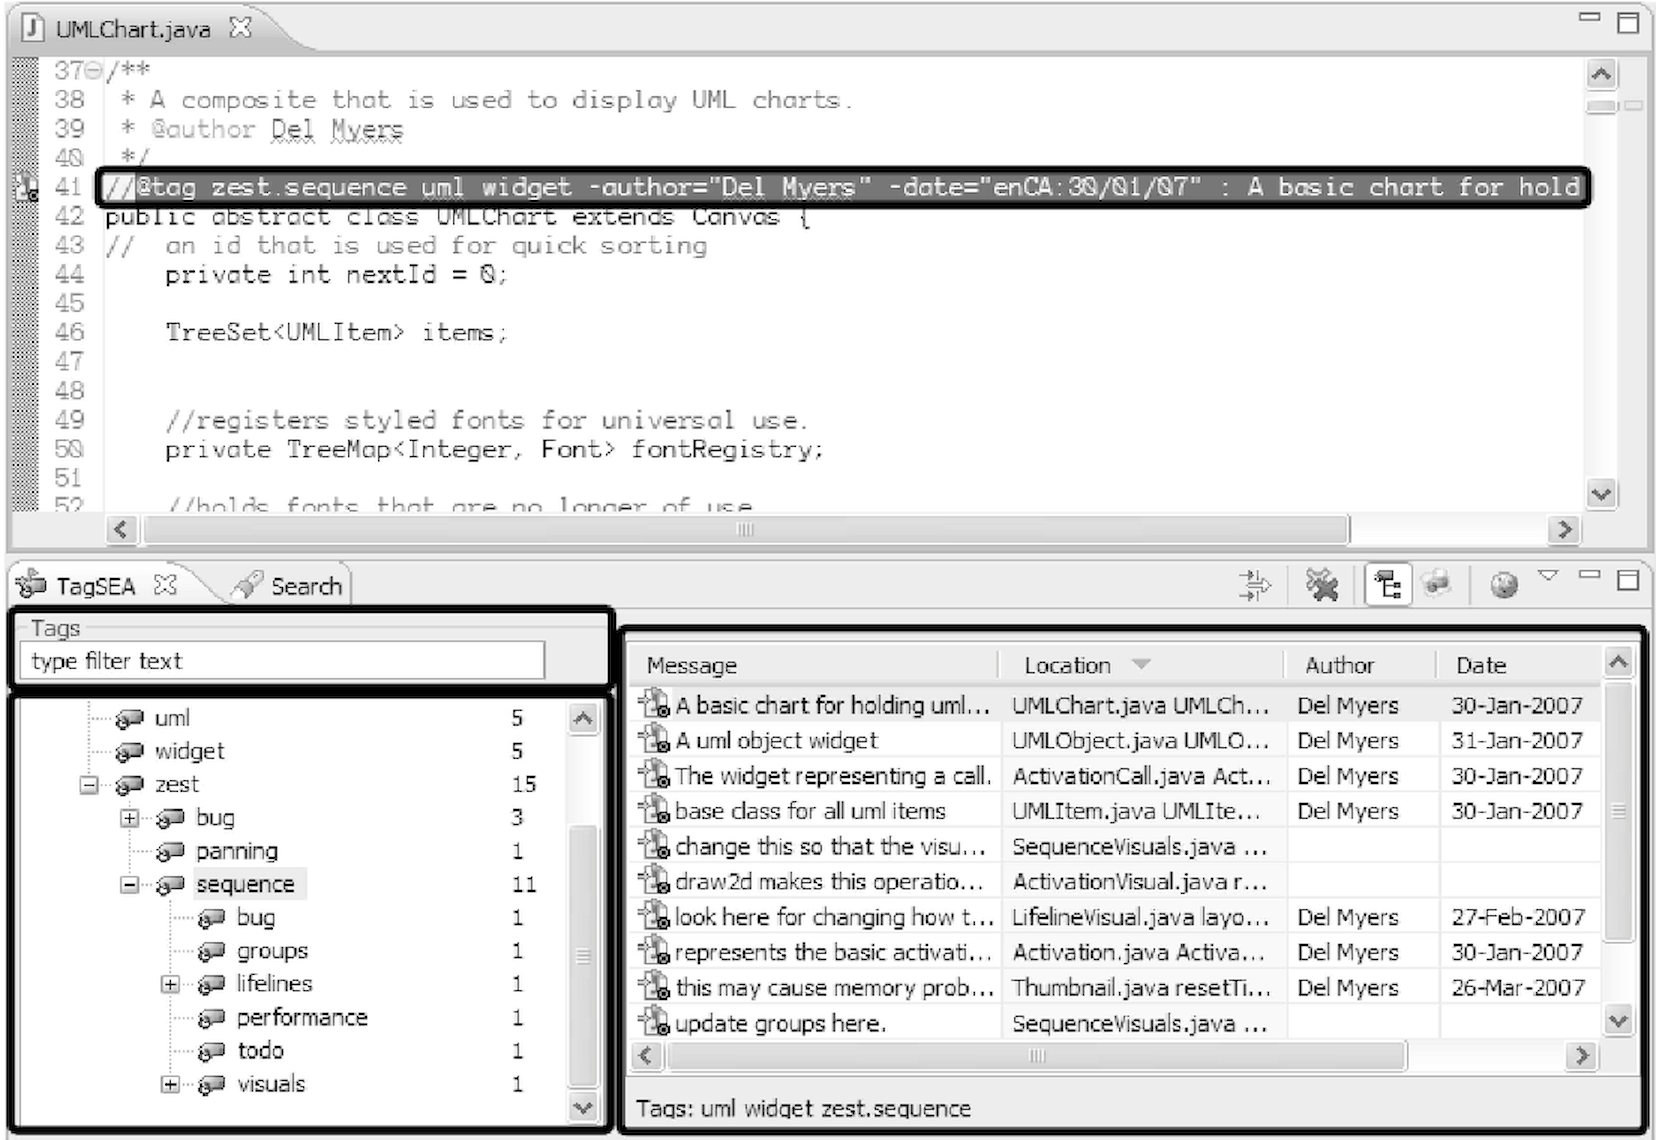
\includegraphics[width=0.8\textwidth]{images/tagsea}
    \caption{TagSEA 0.6.6 used in Eclipse. The highlighted line of code in the upper area shows TagSEA's notation of todo comments. The bottom area shows its extended search based on tags as well as a list of all tags. (Image Source:~\cite{storey_how_2009})}
    \label{fig:tagsea}
\end{figure}
%
TagSEA is implemented as an Eclipse plug-in, which combines a specific notation for waypoints with a custom view for viewing, filtering, and searching them.
Figure~\ref{fig:tagsea} depicts the usage of TagSEA in Eclipse.
Line~\verb|41| in the source code part shows the notation of TagSEA comments.
It becomes immediately visible that although the notation is different from the one used in PEP 350 -- Codetags (also compare Section~\ref{sec:codetags}), one can clearly see that similar properties can be expressed in the comment.
In addition to properties, TagSEA also supports nestable tags (e.g., "zest.sequence", "uml" and "widget" are used in the example in Figure~\ref{fig:tagsea}), which are then represented as a tree.
This feature allows developers to develop project-specific ontologies for managing and refinding todo comments \cite{storey_how_2009}.


\subsubsection{\texttt{todo\_or\_die}}
\label{sec:todo-or-die}
A different approach to handling todo comments is pursued by Justin Searls, one of the core contributors of the Ruby library \texttt{todo\_or\_die} \cite{searls_todo_2023}.
By not depending on any editor features, \texttt{todo\_or\_die} provides exactly one function\footnote{A second function can be utilized to configure the runtime behavior of \texttt{todo\_or\_die}, but it is called once at most.} called \texttt{TodoOrDie}.
Program~\ref{prg:todo-or-die} shows the difference between traditional todo comments (see Line~\verb|2|) and how they are encoded in \texttt{todo\_or\_die} (see Line~\verb|3|).
%
\begin{program}[ht]
\begin{PythonCode}
class UsersController < ApiController
  # TODO: remember to delete after JS app has propagated
  TodoOrDie("delete after JS app has propagated", by: "2019-02-04")
  def show
    redirect_to root_path
  end
end
\end{PythonCode}
\caption{Code example showing the difference between classic todo comments and the application of \texttt{todo\_or\_die}. (Program source:~\cite{searls_todo_2023})}
\label{prg:todo-or-die}
\end{program}
%
Calling the function \texttt{TodoOrDie} does not affect the program's execution, except if the parameter "by" of type date is passed.
In this case, \texttt{TodoOrDie} will raise an error once the class is loaded and this date has already passed.
Instead of passing a date, one can also pass a runtime condition based on the applied class' members.
These two parameters can also be combined, resulting in highly flexible configurations of when todo comments should raise errors.
By making the program crash if certain preconditions are met, \texttt{todo\_or\_die} lifts todo comments from editor space into runtime space.
Instead of seriously affecting the runtime behavior by raising errors, \texttt{todo\_or\_die} can also be configured to, e.g., simply logging the todo comments' messages, although this reduces the effect of its initial idea, namely: making todo comments visible, if intended.


\subsubsection{Todo Comment Viewers}
Bridging the gap between todo comments and software engineering methods can be achieved using, e.g., Tickgit\footnote{\url{https://www.tickgit.com/}}, Catana\footnote{\url{https://catana.dev/}} or imdone\footnote{\url{https://imdone.io/}}.
All three of these tools promise that todo comments can be used as the basis of project management without breaking developer's flows by being code-based.

Tickgit and imdone are direct contenders, both of them being web-based and free for open-source projects.
After analyzing a project for todo comments, users can view, filter, and aggregate them.
Figure~\ref{fig:catana} depicts a screenshot of applying Catana to \href{https://github.com/bemayr/Statecharts.NET}{bemayr/Statecharts.NET} and showing all open \emph{TODO Items}.
Similar to the other presented solutions, todo comments can be tagged with triggers, giving them expiration dates.
%
\begin{figure}
    \centering
    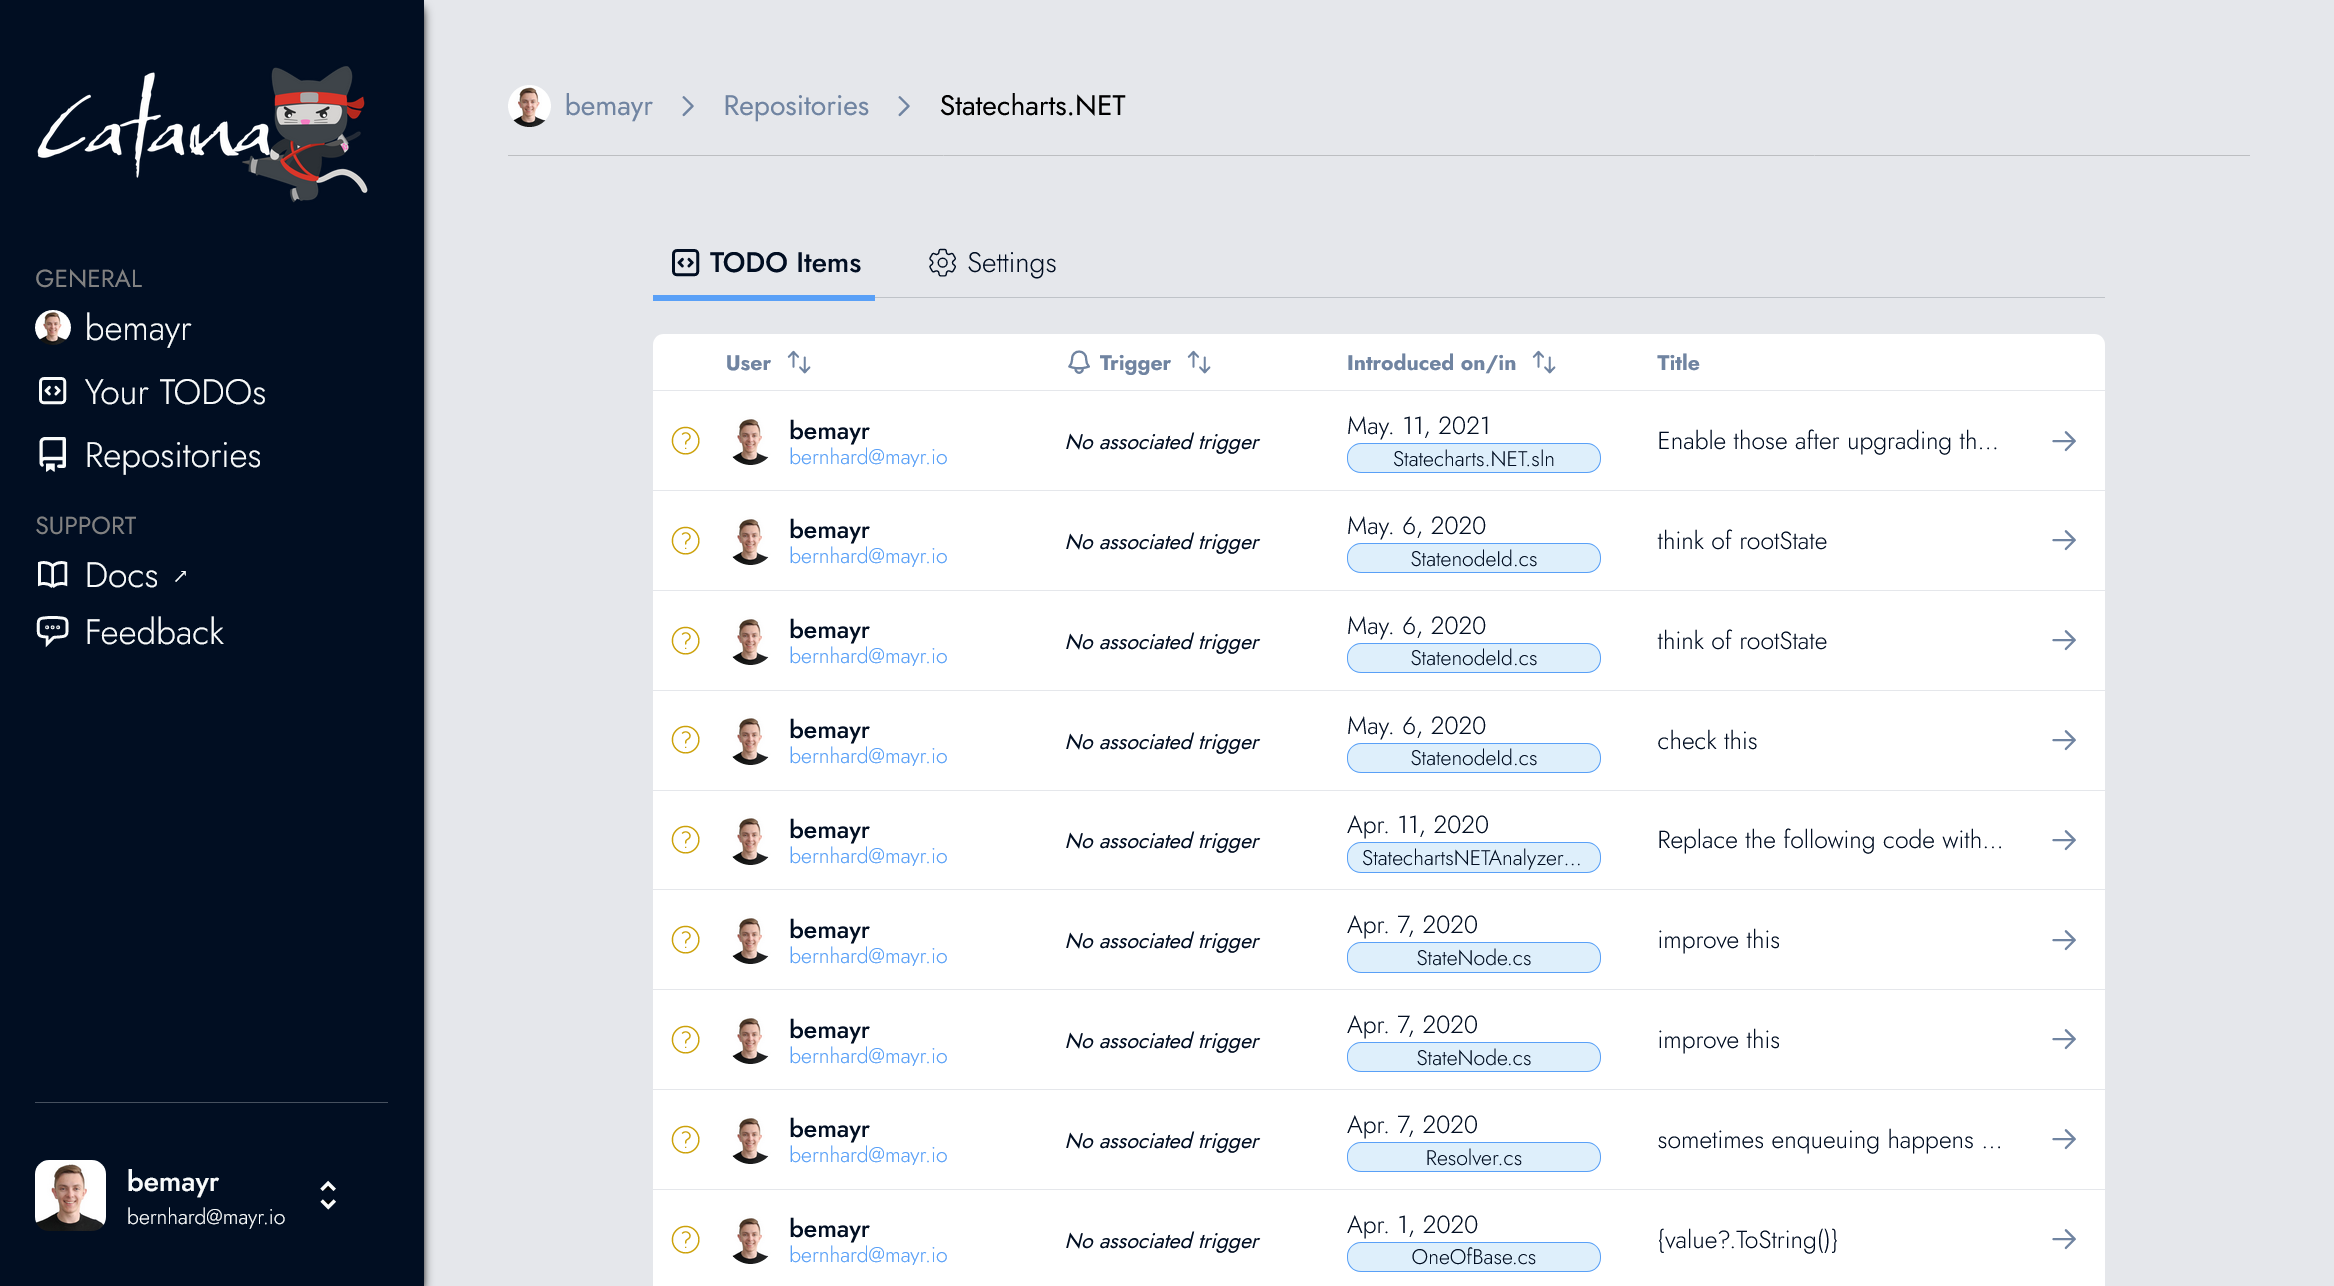
\includegraphics[width=0.9\textwidth]{images/catana}
    \caption{Screenshot of Catana's todo comment list applied to \href{https://github.com/bemayr/Statecharts.NET}{bemayr/Statecharts.NET}.}
    \label{fig:catana}
\end{figure}

Imdone integrates even more project management tools; it runs locally and thus has direct access to the source code.
Based on todo comments, a kanban board is created, which allows their visual editing by providing a drag-and-drop interface (as shown in Figure~\ref{fig:imdone}.
In addition to managing todo comments, imdone also enables developers to create additional cards that are integrated into the Kanban board.
They are stored as plain text files, which allows them to be version-controlled together with the program's source code.
%
\begin{figure}
    \centering
    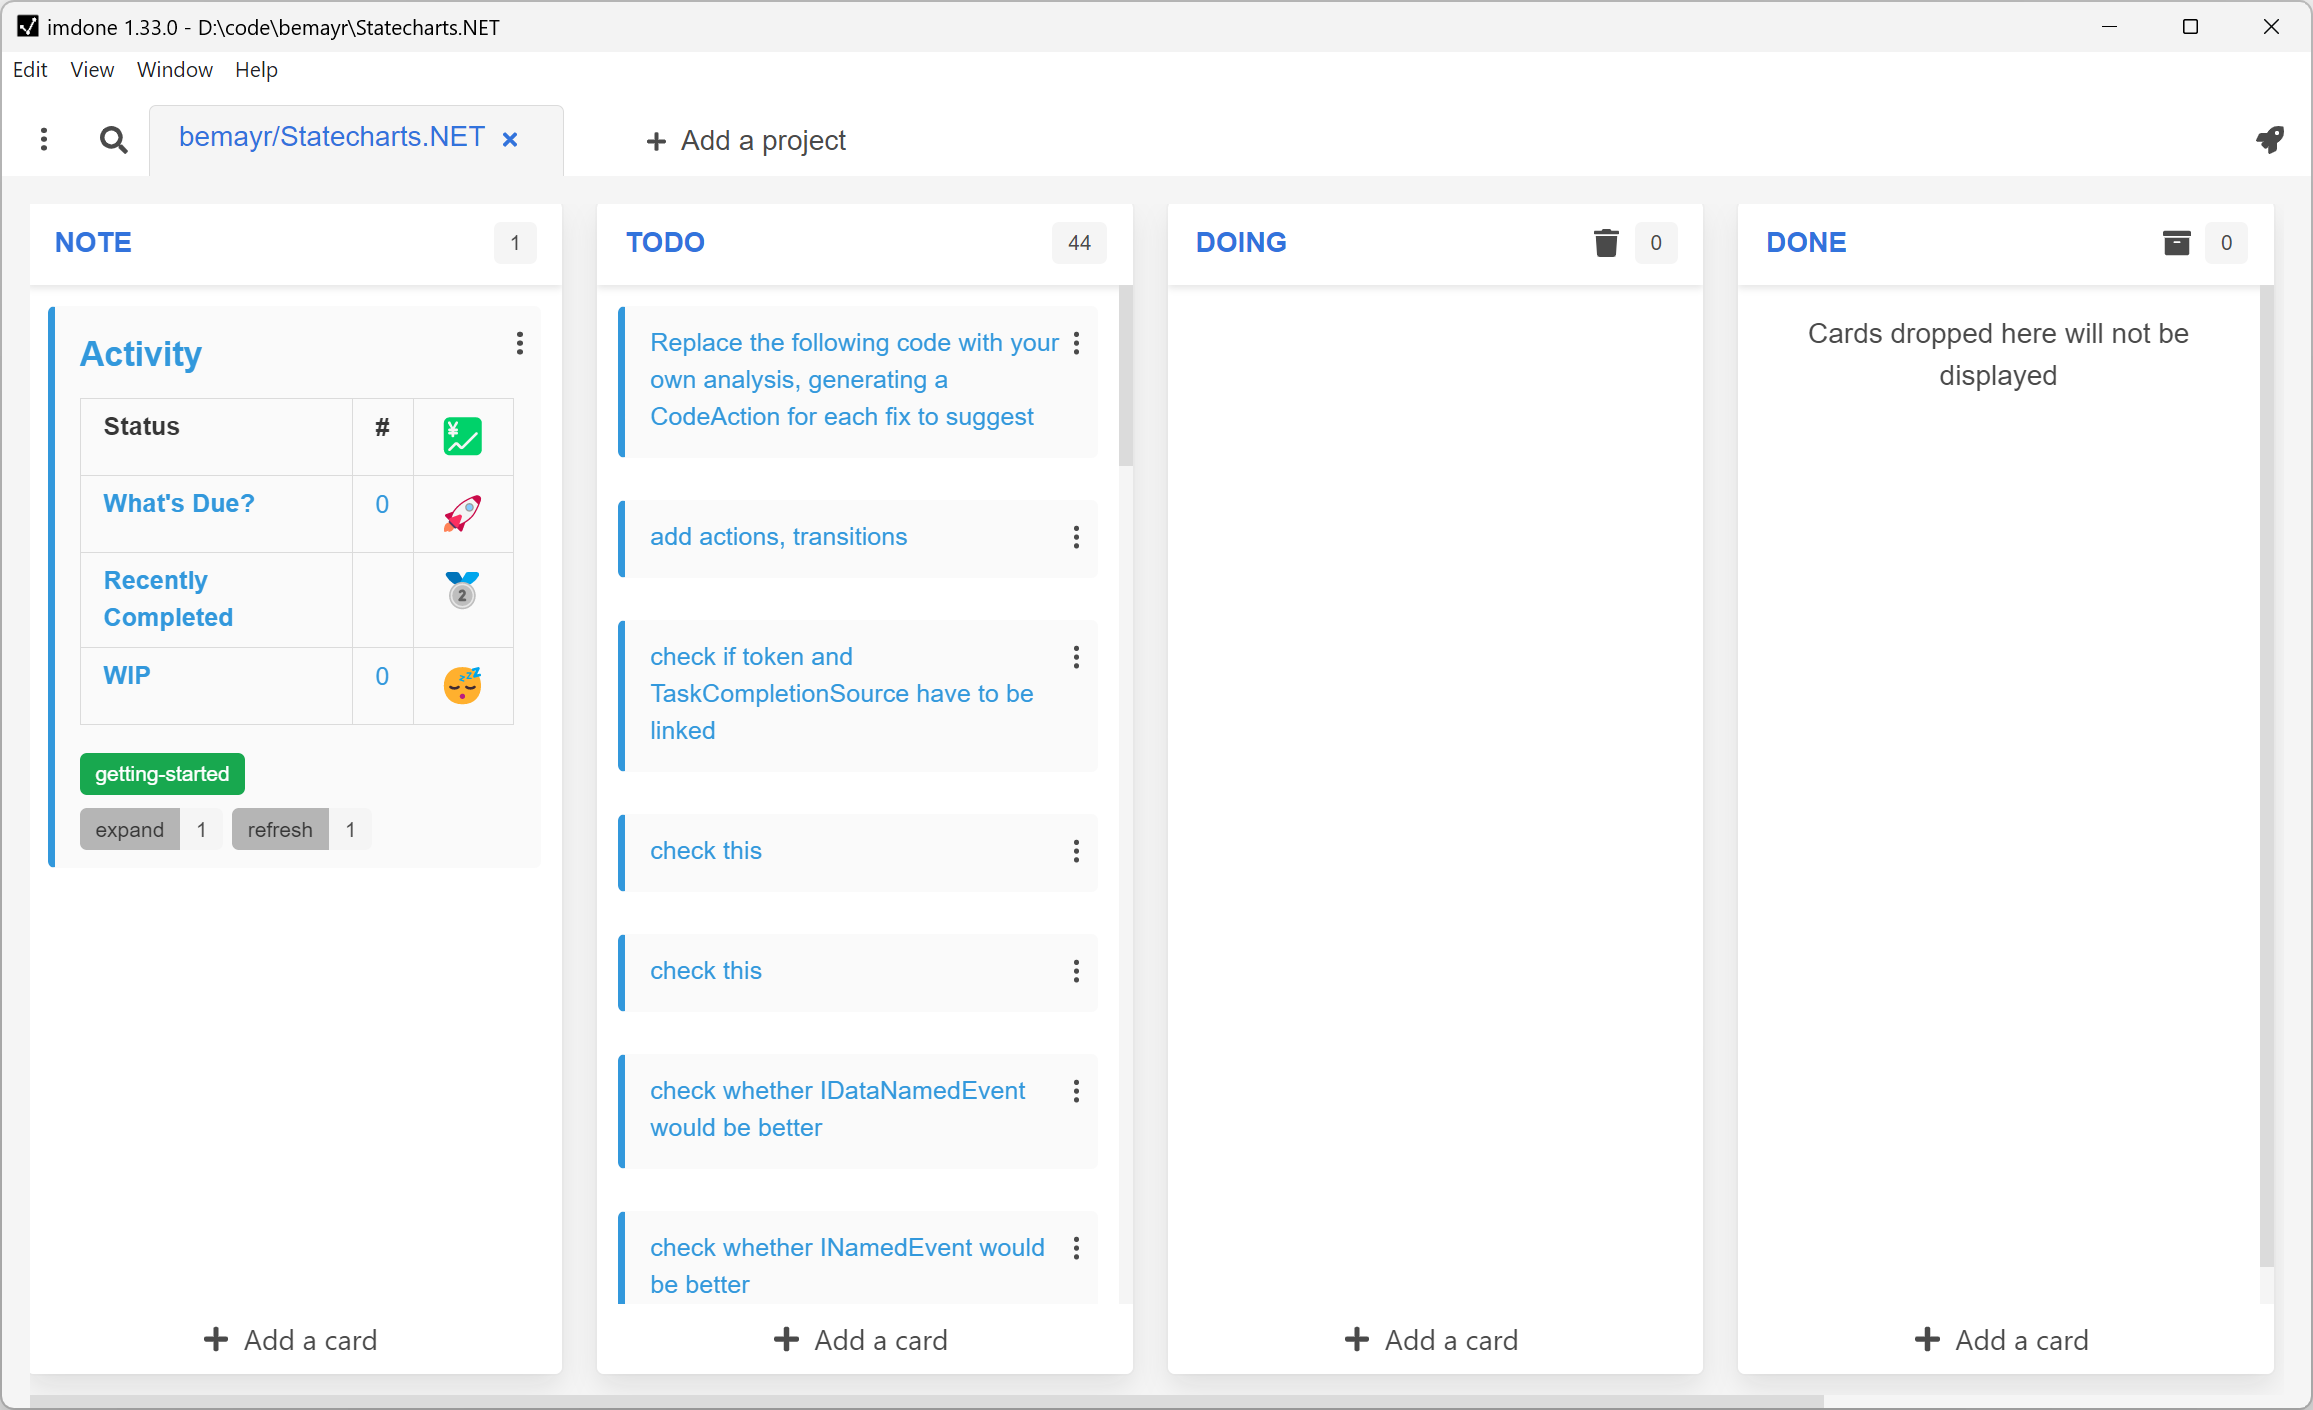
\includegraphics[width=0.9\textwidth]{images/imdone}
    \caption{Imdone's kanban view applied to \href{https://github.com/bemayr/Statecharts.NET}{bemayr/Statecharts.NET} showing the uncompleted todo comments.}
    \label{fig:imdone}
\end{figure}

Regarding the applicability of the presented tools, their application in larger projects remains questionable, but for smaller projects or single developers trying to replace todo lists, these tools can provide high value.
According to imdone's landing page, this tool is used at companies such as Microsoft, Oracle and Intel.

\subsubsection{Editor Features}
\label{sec:todo-comments-ide-features}
Various integrated development environments help with growing numbers of todo comments.
Visual Studio provides the task list window \cite{hogensen_use_2019}, which shows all todo comments in a list.
By default, it includes comments starting with "HACK", "TODO", "UNDONE", and "UnresolvedMergeConflict", although this list can be customized.
JetBrains' \CS IDE Rider offers a similar feature called TODO window \cite{jetbrains_todo_2023}.
Figure~\ref{fig:rider-todo-list} shows a screenshot of this feature.
In addition to customizable todo comments, Rider also shows the usage of \texttt{NotImplementedException}s, which can act as markers for incomplete programs (see Section~\ref{sec:simulating-holes}).
%
\begin{figure}
    \centering
    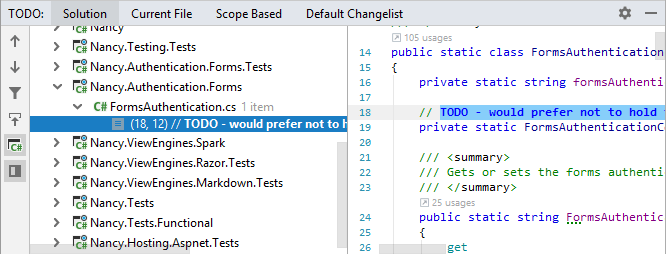
\includegraphics[width=0.7\textwidth]{images/rider-todo-window}
    \caption{JetBrains Rider's TODO window. (Image source:~\cite{searls_todo_2023})}
    \label{fig:rider-todo-list}
\end{figure}

Modern IDEs enable developers to extend them by integrating plug-ins.
Various plug-ins regarding the usage of todo comments have been developed, the following list describes the features for a few of them:
\begin{description}
  \item[Warn About TODOs] is developed by Matt Lacey \cite{lacey_warn_2023}. This Visual Studio Extension tries to prevent the rotting of todo comments by lifting them from editor space into compilation space. Depending on its configuration, todo comments get reported as warnings or error messages in Visual Studio's error list instead of its task list, highlighting their importance.
  \item[Todo Tree] adds the functionality of the aforementioned task list (Visual Studio) or todo window (Rider) to Microsoft's Visual Studio Code Editor \cite{scott_todo_2023}. By adding plug-ins, Visual Studio Code can be turned from an editor into a full-fledged development environment. Todo Tree enables developers to view information regarding their todo comments in various panes. It is highly configurable and can also highlight todo comments in the code.
  \item[TODO Highlight] If one solely wants to highlight todo comments for greater visual attention, the Visual Studio Code extension TODO Highlight does precisely that \cite{wayou_vscode_2023}. Styles and keywords can be configured, and the plug-in respects the currently used theme.
  \item[todo-comments.nvim] is a plug-in for the neovim editor, which provides roughly the same features as Todo Tree for the neovim editor \cite{lemaitre_todo_2023}. It is configurable and provides highlighting capabilities as well as filterable list views.
\end{description}


\section{Languages with native Holes support}
\label{sec:languages-with-native-holes-support}
Continuing with the next way of tackling complexity as described in Section~\ref{sec:tackling-complexity}, the concept of holes exists natively in a few languages.
Although they are sometimes called goals, their main purpose is to aid developers by turning the act of programming into an incremental fill-in-the-hole exercise.
As described in Section~\ref{sec:introducing-hole-driven-development} Hole-Driven Development is loosely based on programming concepts like Type-Driven Development \cite{brady_type-driven_2017} or Test-Driven Development \cite{mccracken_digital_1957} and describes how programming can look like if developers are guided by holes.
In this section, we will look at hole implementations in existing programming languages.

\subsubsection{Coq}
Coq is an interactive theorem prover that supports dependent types \cite{the_coq_development_team_proof_2023}.
Developers can formalize mathematical concepts, while Coq helps them to generate machine-checked proofs of theorems interactively.
In contrast to proofs conducted by humans, machine-checked proofs give users much more confidence.
According to the Coq reference manual: "Users generate proofs by entering a series of tactics that constitute steps in the proof." \cite{the_coq_development_team_proof_2023}
Coq also allows users to extract verified programs to programming languages such as OCaml and Haskell.

In terms of hole-driven development, Coq is of interest due to its proof mode.
This proof mode is used to prove theorems.
A proof's state consists of one or more unproven goals.
Reaching these goals can be accomplished by applying tactics \cite{redmon_coq_2021} based on the proof's local context (e.g., hypotheses, variables, and local definitions) and the global environment (e.g., definitions and proven theorems).

\begin{program}[ht]
\begin{GenericCode}
Goal exists n, n = 0.
    1 goal
      
      ============================
      exists n : nat, n = 0
eexists ?[n].
    1 focused goal (shelved: 1)
      
      ============================
      ?n = 0
Show n.
    goal n is:
      
      ============================
      nat
\end{GenericCode}
\caption{Using goals in Coq's proof mode. (Program source:~\cite{the_coq_development_team_proof_2023})}
\label{prg:coq-goals}
\end{program}

As shown in Program~\ref{prg:coq-goals}, proving theorems is accomplished by interactively iterating on goals and hypotheses.
Line~\verb|1| states the goal, such as there exists a number \verb|n| that equals 0.
Goals in Coq are incomplete parts of the intended proof, which must be fulfilled; thus, they are holes.
Line~\verb|2| displays that there is one open goal, while Line~\verb|5| shows the conclusion of this goal.
In Line~\verb|6|, we apply the tactic \verb|eexists|, which creates a focused goal called \verb|n|.
Coq allows goals to be shelved and focused so that developers can manage the existence of multiple goals.
Line~\verb|11| displays the goal \verb|n|, showing that this goal has to be proven using a natural number (Line~\verb|15|).

This interactive process highlights how holes (or goals in Coq's terms) can support reducing cognitive load (compare Section~\ref{sec:cognitive-load}) by enabling a back-and-forth between bottom-up and top-down problem-solving strategies (compare Section~\ref{sec:programming-as-complex-problem-solving}).

\subsubsection{Agda}
Similar to Coq, Agda is another dependently typed proof assistant, but instead of constructing proofs using tactics, they are written in a functional programming style \cite{knispel_agda_2020}.
In addition, Agda also supports the concept of holes, sometimes also called goals \cite{the_agda_team_holes_2023}.

Program~\ref{prg:agda-holes} shows the usage of holes and interactive proving in Agda \cite{the_agda_team_holes_2023}.
In Line~\verb|1|, we define the first clause of proving associativity with a right-hand side of \verb|?|, which indicates a hole.
After reloading the file and entering interactive proving mode, Agda turns \verb|?| into \verb|{ }0| (see Line~\verb|5| of Program~\ref{prg:agda-holes}), which is now a hole and "stands as a placeholder for a part of the program that is still incomplete and can be refined or resolved interactively" \cite{the_agda_team_holes_2023}.
Agda automatically assigns numbers to the holes.
Agda also knows how natural numbers are represented and therefore is able to split Line~\verb|5| to Lines~\verb|9| and \verb|10| when instructed to case-split on variable \verb|x|.
Note how the Agda system introduced the cases \verb|zero| and \verb|(suc x)| for \verb|x| as well as added a new hole in Line~\verb|10| called \verb|{ }1|.
Getting rid of holes is as simple as replacing them with their implementation, as Line~\verb|14| shows compared to Line~\verb|9|, which uses the term \verb|refl| denoting \emph{reflexivity}.
We will stop here because proving associativity is not the goal of this thesis, but this example shows how holes can be used to de-compose and compose proofs in Agda.

\begin{program}[ht]
\begin{GenericCode}
+-assoc-proof x y z = ?

=== reload the file to enter interactive proving mode ===

+-assoc-proof x y z = { }0

=== case-splitting on x ===

+-assoc-proof zero y z = {  }0
+-assoc-proof (suc x) y z = {  }1

=== applying reflexivity to hole 0 ===

+-assoc-proof zero y z = refl
+-assoc-proof (suc x) y z = {  }1
\end{GenericCode}
\caption{Using holes and case-splitting in Agda. (Program source:~\cite{the_agda_team_holes_2023})}
\label{prg:agda-holes}
\end{program}

\subsubsection{Haskell}
The most widely used and general-purpose programming language that supports holes is Haskell \cite{tiobe_software_bv_tiobe_2023, stack_overflow_stack_2023}.

\cite{gamari_haskell_2019}
\cite{gissurarson_suggesting_2018}
\cite{redmond_toward_2021}

While Haskell is the most general purpose 
\todo[inline,color=blue!40]{maybe do some research regarding Liquid Haskell}
\todo[inline]{compiler flag that allows running incomplete programs}

\begin{program}[ht]
\begin{GenericCode}
module FreeMonad where

data Free f a
  = Pure a
  | Free (f (Free f a))

instance Functor f => Monad (Free f) where
  return a     = Pure a
  Pure a >>= f = f a
  Free f >>= g = Free _
\end{GenericCode}
\caption{Using holes and case-splitting in Agda. (Program source:~\cite{the_agda_team_holes_2023})}
\label{prg:agda-holes}
\end{program}

\begin{program}[ht]
\begin{GenericCode}
Found hole `_' with type f (Free f b)

Relevant bindings include
  >>= :: Free f a -> (a -> Free f b) -> Free f b
    (bound at holes.hs:28:3)
  f :: f (Free f a) (bound at holes.hs:29:8)
  g :: a -> Free f b (bound at holes.hs:29:14)
In the first argument of `Free', namely `_'
\end{GenericCode}
\caption{Using holes and case-splitting in Agda. (Program source:~\cite{the_agda_team_holes_2023})}
\label{prg:agda-holes}
\end{program}

\subsubsection{Hazel}
%https://www.youtube.com/watch?v=UkDSL0U9ndQ
%the gap problem
%what you start with is a hole
%what should we fill this hole with (in-class)
%regarding machine learning: having a theory of incomplete programs allows us to do it this way
%splicing: putting holes inside text

\begin{figure}
    \centering
    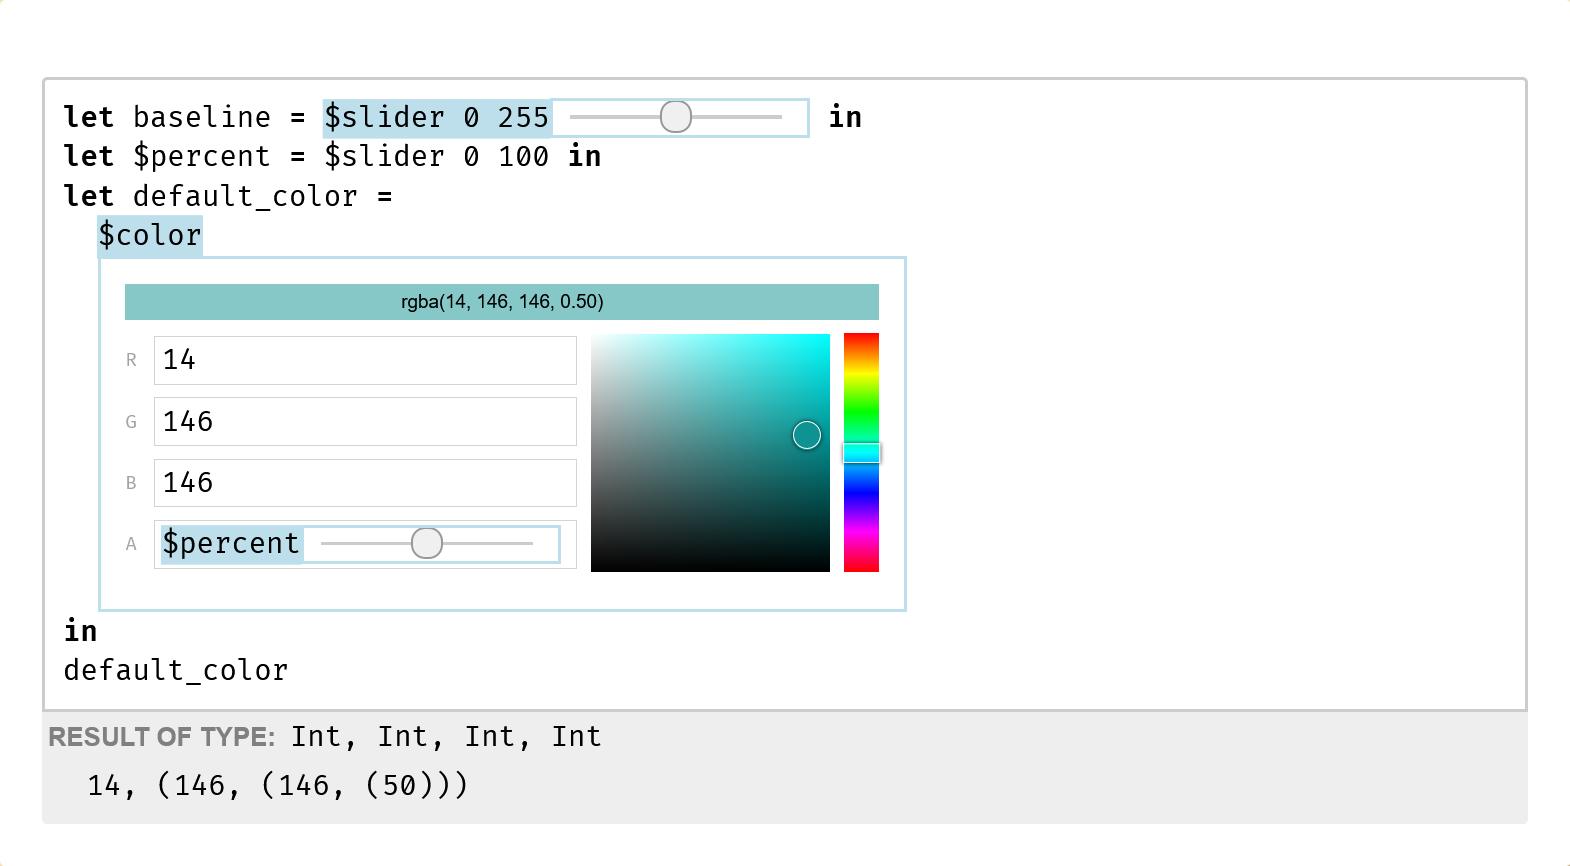
\includegraphics[width=0.7\textwidth]{images/hazel}
    \caption{Using Livelits to fill holes visually in Hazel. (Image source:~\cite{omar_filling_2021})}
    \label{fig:hazel-livelits}
\end{figure}

\subsubsection{Idris}

\section{Simulating Holes in other Languages}
\label{sec:simulating-holes}
By reducing the concept of holes as defined in the previously seen statically typed functional languages to its core, one could argue that the idea of using holes also exists in various other languages.
Providing means of writing incomplete code is very helpful for quickly iterating on unfinished code.
As such, this aspect of holes already found its way into general-purpose programming languages, albeit without the compiler support provided by the languages mentioned in Section~\ref{sec:languages-with-native-holes-support}.
This section will present some of these ad-hoc solutions and show their usage.

\subsubsection{\CS}
One widely used way of writing incomplete \CS\-code that can still be compiled is using \texttt{NotImplementedException} \cite{microsoft_notimplementedexception_2020} for indicating that a piece of code is not yet implemented or "still in development" \cite{microsoft_notimplementedexception_2020}.
The constructor accepts an optional message parameter, which can be used to pass a textual description of the missing implementation.
As this exception indicates missing functionality, it should not be handled using \texttt{try/catch}, but instead, surface at runtime and crash the program to indicate missing parts.
When generating code, IDEs (e.g., Visual Studio) insert \texttt{throw new NotImplementedException()} into method stubs, signaling that these methods still need to be implemented.

Another exception class that sometimes gets confused is \texttt{NotSupportedException}.
As its name indicates, this method should not be used for incomplete code but for cases where certain functionality is not supported.
\texttt{NotSupportedException} should be used carefully, as its usage is a high indicator for breaking either the Liskov substitution principle or the interface segregation principle \cite{patrik_liskov_2017}.

%\todo[inline]{dynamic}: %https://learn.microsoft.com/en-us/dotnet/csharp/advanced-topics/interop/using-type-dynamic

\subsubsection{Java}
Prior to implementing Hazel, \citeauthor{omar_active_2012} worked on adding \emph{active code completion} for Java \cite{omar_active_2012}.
Active code completion describes an architecture that allows library developers to enhance their libraries by enabling interactive and highly specialized user interfaces for generating code.
In Graphite, the Eclipse IDE-plugin developed by \citeauthor{omar_active_2012}, these user interfaces are called \emph{palettes}; they can be distributed alongside libraries and enhance traditional auto-completion in editors \cite{omar_active_2012}.
While traditional auto-completion approaches provide a list of text-based suggestions for what piece of code might follow, palettes allow this completion panel to include a custom domain-specific user interface, as seen in Figure~\ref{fig:graphite-active-code-completion}.

\begin{figure}[ht]
    \centering
    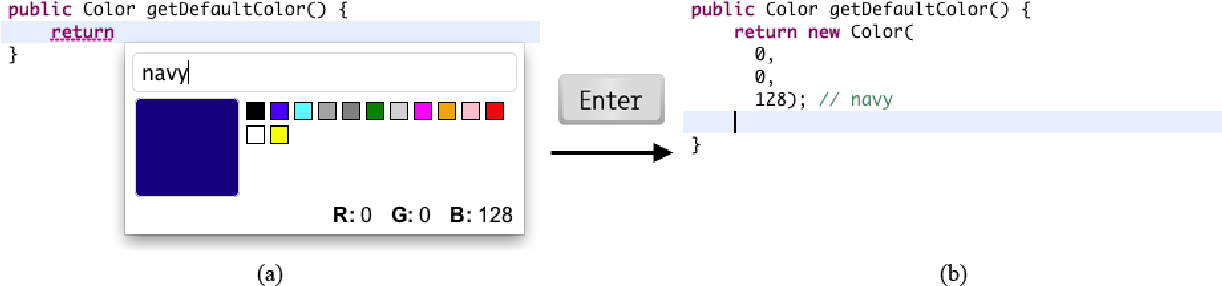
\includegraphics[width=0.85\textwidth]{images/active-code-completion}
    \caption{Example of Graphite's active code completion IDE plug-in. (Image source:~\cite{omar_active_2012})}
    \label{fig:graphite-active-code-completion}
\end{figure}

Part \emph{(a)} of Figure~\ref{fig:graphite-active-code-completion} shows that if an empty expression is encountered that matches the type of a registered palette, the IDE shows a visual user interface for filling this expression.
Viewing these empty expressions as holes, one can argue that for all empty expressions that match the type of an existing palette, a hole is implicitly created, which can be filled using a specialized user interface.
Part \emph{(b)} of Figure~\ref{fig:graphite-active-code-completion} shows the code generated by selecting a color.

Before implementing Graphite, \citeauthor{omar_active_2012} surveyed 473 professional developers regarding their experiences and opinions regarding code completion \cite{omar_active_2012}.
These professional developers described one interesting aspect regarding the usage of palettes and prototypes by explaining that using "palettes that generate constant data may be most useful in the prototyping phase. It can be noted that when transitioning from a prototype to production-quality software, the code generated by a palette or tool may be used as a template to be refactored as needed." \cite{omar_active_2012}

\subsubsection{Scala}
Another textual approach to simulating holes was pursued by Martin Odersky, the creator of the Scala language.
After discussing it with the community and a few design iterations, he added \texttt{???} to Predef, Scala's standard library \cite{odersky_adding_2011}.
In his initial proposal, he argues that instead of defining this method over and over in each project, it would make sense to add it in such a way that it is automatically available in the global scope.
Based on his experience, he suggested that it could be used as a great teaching tool by just telling the class to replace all occurrences of \texttt{???} \cite{odersky_adding_2011}.
Program~\ref{prg:scala-???} shows the full implementation of \texttt{???} including its documentation.
\citeauthor{odersky_adding_2011} decided to throw an \texttt{NotImplementedError} because a missing implementation should behave similarly to a failed assertion.
%
\begin{program}[ht]
\begin{GenericCode}
/** `???` can be used for marking methods that remain to be implemented.
* @throws A `NotImplementedError`
*/
def ??? : Nothing = throw new NotImplementedError
\end{GenericCode}
\caption{Implementation of Scala's \texttt{???} operator. (Program source:~\cite{odersky_adding_2011})}
\label{prg:scala-???}
\end{program}

\subsubsection{Swift}
Simulating hole driven development in Swift can be achieved by using the function \texttt{fatalError()} \cite{martinez_hole_2018}.
Similar to \CS's \texttt{NotImplementedException} or Scala's \texttt{???}-operator it can be used to mark a piece of code as incomplete.
Because of \texttt{fatalError()} returning \texttt{Never}, it can be used instead of any expression in a Swift program.
\texttt{Never} is a bottom type, which is compatible with all possible types.

\subsubsection{Rust}
Similar to \CS, Scala, and Swift, the standard library of Rust contains macros for marking code as "under development".
Rust uses two macros called \texttt{!todo()} \cite{the_rust_project_developers_todo_2023} and \texttt{!unimplemented()} \cite{the_rust_project_developers_unimplemented_2023} with slightly different semantics.
While the former (\texttt{!todo()}) conveys the intention of "not yet implemented", the latter (\texttt{!unimplemented()}) denotes no intention of a future implementation at all.
Regarding the usage of the \texttt{!todo()}-macro, the official Rust docs explain: "This can be useful if you are prototyping and just want a placeholder to let your code pass type analysis." \cite{the_rust_project_developers_todo_2023}

\subsubsection{TypeScript}
One feature of TypeScript that can be interpreted in the light of hole-driven development is the gradual refinement of types using \texttt{any} and \texttt{unknown} \cite{baumgartner_typescript_2023}.
Instead of applying the concept of holes at the runtime level, this idea is aimed at the compilation level.

TypeScript, being a superset of JavaScript, enables types to be specified only optionally \cite{baumgartner_typescript_2023}.
This setting can be configured in \texttt{\seqsplit{tsconfig.json}} using the property \texttt{\seqsplit{noImplicitAny}}.
If it is set to \texttt{false}, types do not have to be provided, which hugely helps when introducing TypeScript in legacy code bases.
Another use case is the fast-paced development of prototypes, where fast development cycles are favored over type safety.
Once developers introduce types, they can use \texttt{any} or \texttt{unknown} as a starting point.
Both of these types are top types, which means that every value is compatible with them, while "\texttt{any} allows you to do everything, \texttt{unknown} allows you to do nothing." \cite{baumgartner_typescript_2023}
Both types enable developers to start with a broad, "fits-all" type, which can be gradually refined over time by making it more explicit.
This process of gradual refinement can be seen as hole-driven development, where the incomplete, experimental hole is provided at first and gradually improved to provide proper type safety.

\subsubsection{\LaTeX}
Even this thesis was written using a hole-driven approach.
Various \LaTeX-packages (e.g. todonotes\footnote{\url{https://ctan.org/pkg/todonotes}}, easy-todo\footnote{\url{https://ctan.org/pkg/easy-todo}}, fixmetodonotes\footnote{\url{https://ctan.org/pkg/fixmetodonotes}}, todo\footnote{\url{https://ctan.org/pkg/todo}}, and fixme\footnote{\url{https://ctan.org/pkg/fixme}} can be used to create holes in a document.
These packages allow the insertion of meta-notes into documents.
They do not belong to the document but are used during its development or review phase.
Enabling discussions about the document in the document, these packages improve collaborative activities.
E.g., Martin Dagleish commented on the todonotes-packages via ctan: "This package is excellent, not only for working on your own but also for working together because you can mark passages in different colors for other people, e.g., for rewriting, information, ..." \cite{dagleish_comment_2021}.
An interesting aspect of the \emph{fixme}-package is its concept of modes.
Everything works as expected in draft mode, once final mode is activated, the behavior changes: remaining notes now generate errors, thus breaking the build of the document and indicating that these notes must be resolved to finish the document.
The following todo comment explains how this thesis was approached using the concept of holes while also showing how todo comments look when using \verb|\todo[inline]{<note_content>}| of the \emph{todonotes} \LaTeX-package:

\vspace{3mm}
\todo[inline]{After creating a document outline, ideas, notes, and references have been assigned to all sections as todo items. Hole after hole, these notes have been turned into prose, while new holes have been introduced for other ideas, cross-references, or missing literature references.}


\section{Properties of Holes}
\label{sec:relevant-properties}
After reviewing existing solutions for holes and hole-like concepts, we will derive a list of their most common properties in this section.
In addition to the properties of well-established holes in statically functional languages (compare Section~\ref{sec:languages-with-native-holes-support}, we introduce properties that we observed while we were looking at the usage of todo comments (compare Section~\ref{sec:tackling-todo-comments} as well as how hole-like concepts (compare Section~\ref{sec:simulating-holes}) are enabled by certain language features.
These properties (prefixed with \emph{HP} for \emph{hole property}) constitute the basis for implementing our proof of concept in \CS (see Chapter~\ref{cha:implementation}):
%
\begin{properties}
    \item The notation of holes should be as concise as possible, which improves writability and reduces visual clutter.\label{hp:concise}
    \item Writing holes should be idiomatic, preserving native language features and concepts, which reduces the learning curve.\label{hp:idiomatic}
    \item Programs containing holes should be executable, thus enabling the ideas of interactive programming.\label{hp:executable}
    \item Holes can be described using (prose) messages; they aid in reminding developers of their thoughts later on.\label{hp:prose-message}
    \item Holes can be marked using custom tags, which enables the creation of custom taxonomies and simplifies their refinding in large codebases.\label{hp:taggable}
    %\item \label{hp:gradually-refinable}
    \item Using holes should be as editor-independent as possible, which enables their usage on as many platforms as possible.\label{hp:editor-independence}
    \item If holes affect runtime behavior, this behavior can be specified, which results in flexibility.\label{hp:runtime-behavior}
    \item Holes produce compiler messages (e.g., warnings or errors) so they are not forgotten or overlooked.\label{hp:compile-warnings}
    \item The severity of a hole's compiler message depends on the compilation or runtime mode; this enables quick prototypes, albeit preventing prototypical code from being released.\label{hp:severity-modes}
    \item Editing holes is supported by editor actions, which improves the usability of handling potential plain text notes.\label{hp:supported-editor-actions}
    \item By extracting type information, implementing a hole can be guided by combining the types of already existing functionality in the code base with a hole's desired type.\label{hp:matchable-via-types}
    \item Holes can be nested, which enables the usage of holes inside other holes.\label{hp:nestable}
    \item By providing capabilities to edit the content of holes visually, they introduce interactivity and experimentation capabilities to programming.\label{hp:visually-editable}
\end{properties}
